\documentclass[twocolumn,a4j]{jarticle}
\usepackage[dvipdfmx]{graphicx}
\usepackage{url}
\usepackage{ascmac}
\usepackage{amsmath, amssymb}
\usepackage{fancyhdr}
\renewcommand{\topfraction}{1.0}
\renewcommand{\bottomfraction}{1.0}
\renewcommand{\dbltopfraction}{1.0}
\renewcommand{\textfraction}{0.01}
\renewcommand{\floatpagefraction}{1.0}
\renewcommand{\dblfloatpagefraction}{1.0}
\setcounter{topnumber}{5}
\setcounter{bottomnumber}{5}
\setcounter{totalnumber}{10}

% 所属と氏名を右寄せにする設定
\makeatletter
  \def\@maketitle{%
  \newpage\null
  %\vskip 2em%
  \begin{center}%
  \let\footnote\thanks
    {\LARGE \@title \par}%
    %\vskip 1.5em%
  \end{center}% 追加
  \begin{center}% 追加
    {\large \@author}%
  \end{center}%
    %\mbox{}\hfill%% 追加
    %{\large
      %\lineskip .5em%
      %\begin{tabular}[t]{r}%
        %\@author
      %\end{tabular}\par}%
    %\vskip 1em%
  \begin{center}% 追加
    {\large \@date}%
  \end{center}%
  %\par\vskip 1.5em
}
\makeatother
\def\vec#1{\mbox{\boldmath $#1$}} 


% 余白の設定
\usepackage[top=20truemm,bottom=20truemm,left=25truemm,right=15truemm]{geometry}


% 箇条書きの行間
\let\olditemize\itemize
\renewcommand{\itemize}{
\olditemize
\setlength{\itemsep}{0.5pt}
\setlength{\parskip}{0pt}
\setlength{\parsep}{0pt}
}

%%%%%%%%%%%%%%%%%%%%%%%%%%%%%%%% 皆さんが書き換えるのはここから %%%%%%%%%%%%%%%%%%%%%%%%%%%%%%%%%%%%%%%

% タイトル
\title{安全運転の持続的な意識づけを促す\\運転操作フィードバック手法に関する研究}
\author{発表者:機械知能システム学専攻 北川 浩行(2332034),k2332034@edu.cc.uec.ac.jp\\
主任指導教員:中村 友昭 准教授,副指導教員:横井 浩史 教授} % 所属,学籍番号,名前
\date{}

%%%%%%%%%%%%%%%%%%%%%%%%%%%%%%%%
% ここの数字をいじってページ数をちょうど1ページに合わせましょう.
\renewcommand{\baselinestretch}{0.73}
%%%%%%%%%%%%%%% ここまで %%%%%%%%%%%%%%%%%

\begin{document}
\maketitle

\def\bq{\begin{equation}}
\def\eq{\end{equation}}
\def\beq{\begin{eqnarray}}
\def\eeq{\end{eqnarray}}
\def\ba{\begin{array}}
\def\ea{\end{array}}
\def\bc{\begin{center}}
\def\ec{\end{center}}
\def\dsum{\sum\limits}
\def\disp{\displaystyle}
\def\ejw{e^{j\omega}}
\def\ejwi{e^{j\omega_{i}}}
\def\e-jwi{e^{-j\omega_{i}}}
\def\dfrac#1#2{\disp{\frac{#1}{#2}}}
\def\teigi{\stackrel{\triangle}{=}}
%\def\b0{\mbox{\boldmath$0$}}
\if0
\def\baa{\mbox{\boldmath$a$}}
\def\bb{\mbox{\boldmath$b$}}
\def\bcc{\mbox{\boldmath$c$}}
\def\bd{\mbox{\boldmath$d$}}
\def\be{\mbox{\boldmath$e$}}
\def\bff{\mbox{\boldmath$f$}}
\def\bg{\mbox{\boldmath$g$}}
\def\bh{\mbox{\boldmath$h$}}
\def\bi{\mbox{\boldmath$i$}}
\def\bj{\mbox{\boldmath$j$}}
\def\bk{\mbox{\boldmath$k$}}
\def\bl{\mbox{\boldmath$l$}}
\def\bm{\mbox{\boldmath$m$}}
\def\bn{\mbox{\boldmath$n$}}
\def\bo{\mbox{\boldmath$o$}}
\def\bp{\mbox{\boldmath$p$}}
\def\bqq{\mbox{\boldmath$q$}}
\def\br{\mbox{\boldmath$r$}}
\def\bs{\mbox{\boldmath$s$}}
\def\bt{\mbox{\boldmath$t$}}
\def\bu{\mbox{\boldmath$u$}}
\def\bv{\mbox{\boldmath$v$}}
\def\bw{\mbox{\boldmath$w$}}
\def\bx{\mbox{\boldmath$x$}}
\def\by{\mbox{\boldmath$y$}}
\def\bz{\mbox{\boldmath$z$}}
\def\bA{\mbox{\boldmath$A$}}
\def\bB{\mbox{\boldmath$B$}}
\def\bC{\mbox{\boldmath$C$}}
\def\bD{\mbox{\boldmath$D$}}
\def\bE{\mbox{\boldmath$E$}}
\def\bF{\mbox{\boldmath$F$}}
\def\bG{\mbox{\boldmath$G$}}
\def\bH{\mbox{\boldmath$H$}}
\def\bI{\mbox{\boldmath$I$}}
\def\bJ{\mbox{\boldmath$J$}}
\def\bK{\mbox{\boldmath$K$}}
\def\bL{\mbox{\boldmath$L$}}
\def\bM{\mbox{\boldmath$M$}}
\def\bN{\mbox{\boldmath$N$}}
\def\bO{\mbox{\boldmath$O$}}
\def\bP{\mbox{\boldmath$P$}}
\def\bQ{\mbox{\boldmath$Q$}}
\def\bR{\mbox{\boldmath$R$}}
\def\bS{\mbox{\boldmath$S$}}
\def\bT{\mbox{\boldmath$T$}}
\def\bU{\mbox{\boldmath$U$}}
\def\bV{\mbox{\boldmath$V$}}
\def\bW{\mbox{\boldmath$W$}}
\def\bX{\mbox{\boldmath$X$}}
\def\bY{\mbox{\boldmath$Y$}}
\def\bZ{\mbox{\boldmath$Z$}}
\fi
\if0
\def\b0{\bf{0}}
\def\bPhi{\mbox{\boldmath$\Phi$}}
\def\bomega{\mbox{\boldmath$\omega$}}
\def\bLambda{\mbox{\boldmath$\Lambda$}}
\def\blambda{\mbox{\boldmath$\lambda$}}
\def\bmu{\mbox{\boldmath$\mu$}}
\def\bnu{\mbox{\boldmath$\nu$}}
\def\bSigma{\mbox{\boldmath$\Sigma$}}
\def\bPhi{\mbox{\boldmath$\Phi$}}
\def\balpha{\mbox{\boldmath$\alpha$}}
\def\bTheta{\mbox{\boldmath$\Theta$}}
\def\btheta{\mbox{\boldmath$\theta$}}
\def\bGamma{\mbox{\boldmath$\Gamma$}}
\def\bPsi{\mbox{\boldmath$\Psi$}}
\def\bDelta{\mbox{\boldmath$\Delta$}}
\def\bPi{\mbox{\boldmath$\Pi$}}
\fi
\makeatletter
\def\lddots{\mathinner{\mkern1mu\raise\p@\vbox{\kern7\p@\hbox{.}}\mkern2mu
\raise4\p@\hbox{.}\mkern2mu\raise7\p@\hbox{.}\mkern1mu}}
\makeatother
\def\argmax{\mathop{\rm argmax}}
\def\baa{{ \boldsymbol a}}
\def\bb{{ \boldsymbol b}}
\def\bcc{{ \boldsymbol c}}
\def\bd{{ \boldsymbol d}}
\def\be{{ \boldsymbol e}}
\def\boldsymbolf{{ \boldsymbol f}}
\def\bg{{ \boldsymbol g}}
\def\bh{{ \boldsymbol h}}
\def\bi{{ \boldsymbol i}}
\def\bj{{ \boldsymbol j}}
\def\bk{{ \boldsymbol k}}
\def\bl{{ \boldsymbol l}}
\def\bm{{ \boldsymbol m}}
\def\bn{{ \boldsymbol n}}
\def\bo{{ \boldsymbol o}}
\def\bp{{ \boldsymbol p}}
\def\bqq{{ \boldsymbol q}}
\def\br{{ \boldsymbol r}}
\def\bs{{ \boldsymbol s}}
\def\bt{{ \boldsymbol t}}
\def\bu{{ \boldsymbol u}}
\def\bv{{ \boldsymbol v}}
\def\bw{{ \boldsymbol w}}
\def\bx{{ \boldsymbol x}}
\def\by{{ \boldsymbol y}}
\def\bz{{ \boldsymbol z}}
\def\bA{{ \boldsymbol A}}
\def\bB{{ \boldsymbol B}}
\def\bC{{ \boldsymbol C}}
\def\bD{{ \boldsymbol D}}
\def\bE{{ \boldsymbol E}}
\def\bF{{ \boldsymbol F}}
\def\bG{{ \boldsymbol G}}
\def\bH{{ \boldsymbol H}}
\def\bI{{ \boldsymbol I}}
\def\bJ{{ \boldsymbol J}}
\def\bK{{ \boldsymbol K}}
\def\bL{{ \boldsymbol L}}
\def\bM{{ \boldsymbol M}}
\def\bN{{ \boldsymbol N}}
\def\bO{{ \boldsymbol O}}
\def\bP{{ \boldsymbol P}}
\def\bQ{{ \boldsymbol Q}}
\def\bR{{ \boldsymbol R}}
\def\bS{{ \boldsymbol S}}
\def\bT{{ \boldsymbol T}}
\def\bU{{ \boldsymbol U}}
\def\bV{{ \boldsymbol V}}
\def\bW{{ \boldsymbol W}}
\def\bX{{ \boldsymbol X}}
\def\bY{{ \boldsymbol Y}}
\def\bZ{{ \boldsymbol Z}}
\def\b0{{\boldsymbol 0}}
\def\bPhi{{\boldsymbol\Phi}}
\def\bomega{{\boldsymbol\omega}}
\def\bLambda{{\boldsymbol\Lambda}}
\def\blambda{{\boldsymbol\lambda}}
\def\bmu{{\boldsymbol\mu}}
\def\bnu{{\boldsymbol\nu}}
\def\bSigma{{\boldsymbol\Sigma}}
\def\bPhi{{\boldsymbol\Phi}}
\def\balpha{{\boldsymbol\alpha}}
\def\bTheta{{\boldsymbol\Theta}}
\def\btheta{{\boldsymbol\theta}}
\def\bGamma{{\boldsymbol\Gamma}}
\def\bPsi{{\boldsymbol\Psi}}
\def\bDelta{{\boldsymbol\Delta}}
\def\bPi{{\boldsymbol\Pi}}

\section{研究の背景と目的}
\vspace*{-0.1cm}
人間は他者とコミュニケーションすることによって,協調行動を学習することができる.
また,自身の状態を記号(言語)で表現し相手に伝達することで,その記号を介して互いの状態を理解し,最適な行動を選択することができる.
このように,記号を介してコミュニケーションを取ることで,互いに理解できる共有された記号が創発される過程を,創発コミュニケーションと呼ぶ.
この創発コミュニケーションを確率的生成モデルで表現した手法として,谷口らによって提案されたメトロポリス・ヘイスティングス名付けゲーム(MHNG)がある\cite{mh1}.
%MH名付けゲームは共有記号の創発の過程を確率的生成モデルで表現した手法であり,相手の観測情報を直接参照することなくエージェント同士が理解できる記号を創発できるモデルである.
%我々はMHNGをマルチエージェント強化学習に応用することで,実環境のロボットを用いたタスクやマルチステップの意思決定を伴う協調タスクを実行する手法をこれまでに提案してきた\cite{ebara}\cite{nakamura}.
筆者はMHNGをマルチエージェント強化学習に応用することで,実環境のロボットを用いた協調タスクを実行する手法を提案した\cite{ebara}.さらに,これを応用したマルチステップの意思決定を伴う協調タスクを実行する手法が提案された\cite{nakamura}.
しかし,これらの手法は離散的な状態・行動しか扱うことができないため,複雑なタスクへの応用が困難という問題がある.
そこで本稿では,MHNGと深層強化学習を組み合わせることで,より複雑な協調行動を学習できるモデルを提案する.
実験では,2体のエージェントが,MHNGにより創発されたメッセージを介してコミュニケーションすることで,協調行動の学習が可能であることを示す.

%%%%%%%%%%%%%%%%%%%%%%%%%%%%%%%%%%%%%%%%%%%%%%%%%%%%%%%%%%%%%%%%%%%%%%%%%%%%%%%%%%%%%%%%%

\section{研究の方法}
\label{method}
図\ref{fig:model}が提案手法のモデル構造であり,各変数の説明は表\ref{tbl:params}の通りである.
2つのSoft Actor Criticモデルをエージェントとし,それぞれがメッセージを介して協調行動を学習する.

\subsection{MHNGによるメッセージの創発}
\label{2.1}
2体のエージェントが協調行動するためには,互いの状態を伝達するための記号が必要となる.
ここで,$m^t$という潜在変数から互いの状態$s^t_{A}, s^t_{B}$と協調行動の報酬$r^t_{m}$ が生成されると仮定する.
このモデルでは,$m^t$は互いの状態の決定に影響を与えるため,この潜在変数$m^t$はメッセージと考えることができる.
メッセージを創発するために,各ステップのエージェントの状態$s^t_{A}, s^t_{B}$と協調行動の報酬$r^t_{m} $からメッセージ$m^t$を推論する.
%
\begin{eqnarray}
m^t \sim p(\cdot | s^t_{A}, s^t_{B},  r^t_{m} ) \label{eq:message}
\end{eqnarray} 
%
しかし,式(\ref{eq:message})は自身からは観測できない相手の状態が含まれており,直接計算することができない.
そこで,文献\cite{mh1}と同様にMHNGを用いることで,互いに独立してメッセージを推論する.
まずエージェントAが次式のように,$s^t_A$と$r^t_A$をもとに$m^{t*}$を生成し,Bに提案する.
%
\begin{equation}
m^{t*} \sim p(\cdot | s^t_{A}, r^t_{m}) \label{eq:porpose_prob}
\end{equation}
%
Bは提案された$m^{t*}$を自身の予測に基づき,次式の受理確率に従って受理または棄却する.
%
\begin{equation}
r =  \frac{p(m^{t*}|s^t_{B}, r^t_{m})}{p(m^t|s^t_{B}, r^t_{m})} \label{acception}
\end{equation}
%
$m^t$は現在のメッセージを表す.
式(\ref{acception})より,Aから提案された$m^{t*}$の受理確率は,Bのパラメータのみから計算することができる.
つまり,相手の状態を直接観測することなく,メッセージの受理/棄却を判断することができる.

以上の手順を役割を交代しながら繰り返し,最適なメッセージを推論する.
このメッセージのやり取りをするコミュニケーションによって,2体のエージェントが,両者の状態に応じて最適な行動を選択することができる.

%
\begin{figure}[t]
\centering
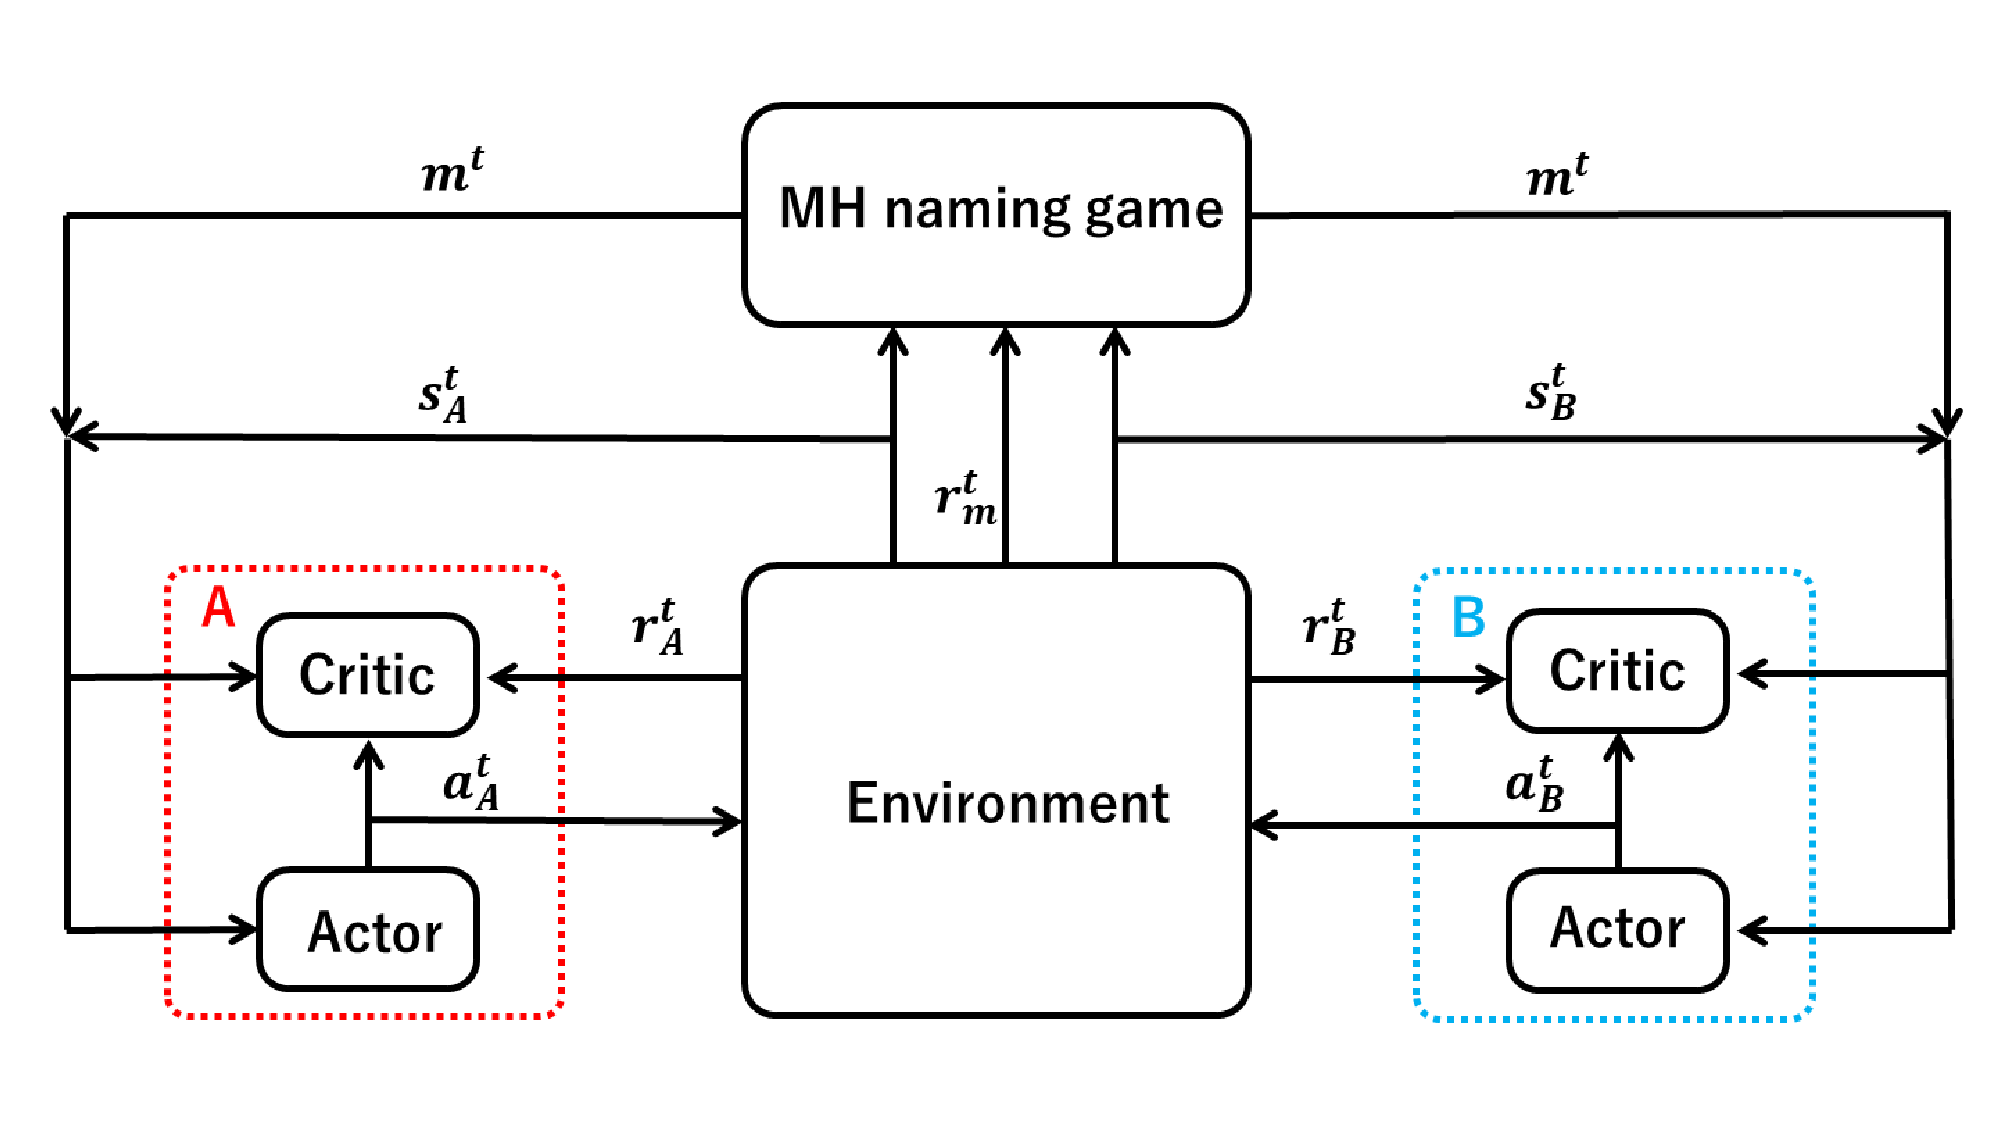
\includegraphics[scale=0.23]{fig/model.pdf}
\caption{提案モデルの概要図}
\label{fig:model}
\end{figure}

%
\begin{table}[t]
  \caption{各変数の詳細}
  \label{tbl:params}
  \centering
  \small
  \begin{tabular}{|c|l|} \hline

    $s^t_{A}, s^t_{B}$	&各エージェントの状態 \\ \hline
    $a^t_{A}, a^t_{B}$	&各エージェントの行動 \\ \hline
    $r^t_{A}, r^t_{B}$	&各エージェントの報酬 \\ \hline
    $r^t_{m}$	&協調行動の報酬 \\ \hline
   $m^t$		&エージェント間でやり取りされるメッセージ \\ \hline
  \end{tabular}
\end{table}
%

\begin{figure*}[t]
	\begin{center}
	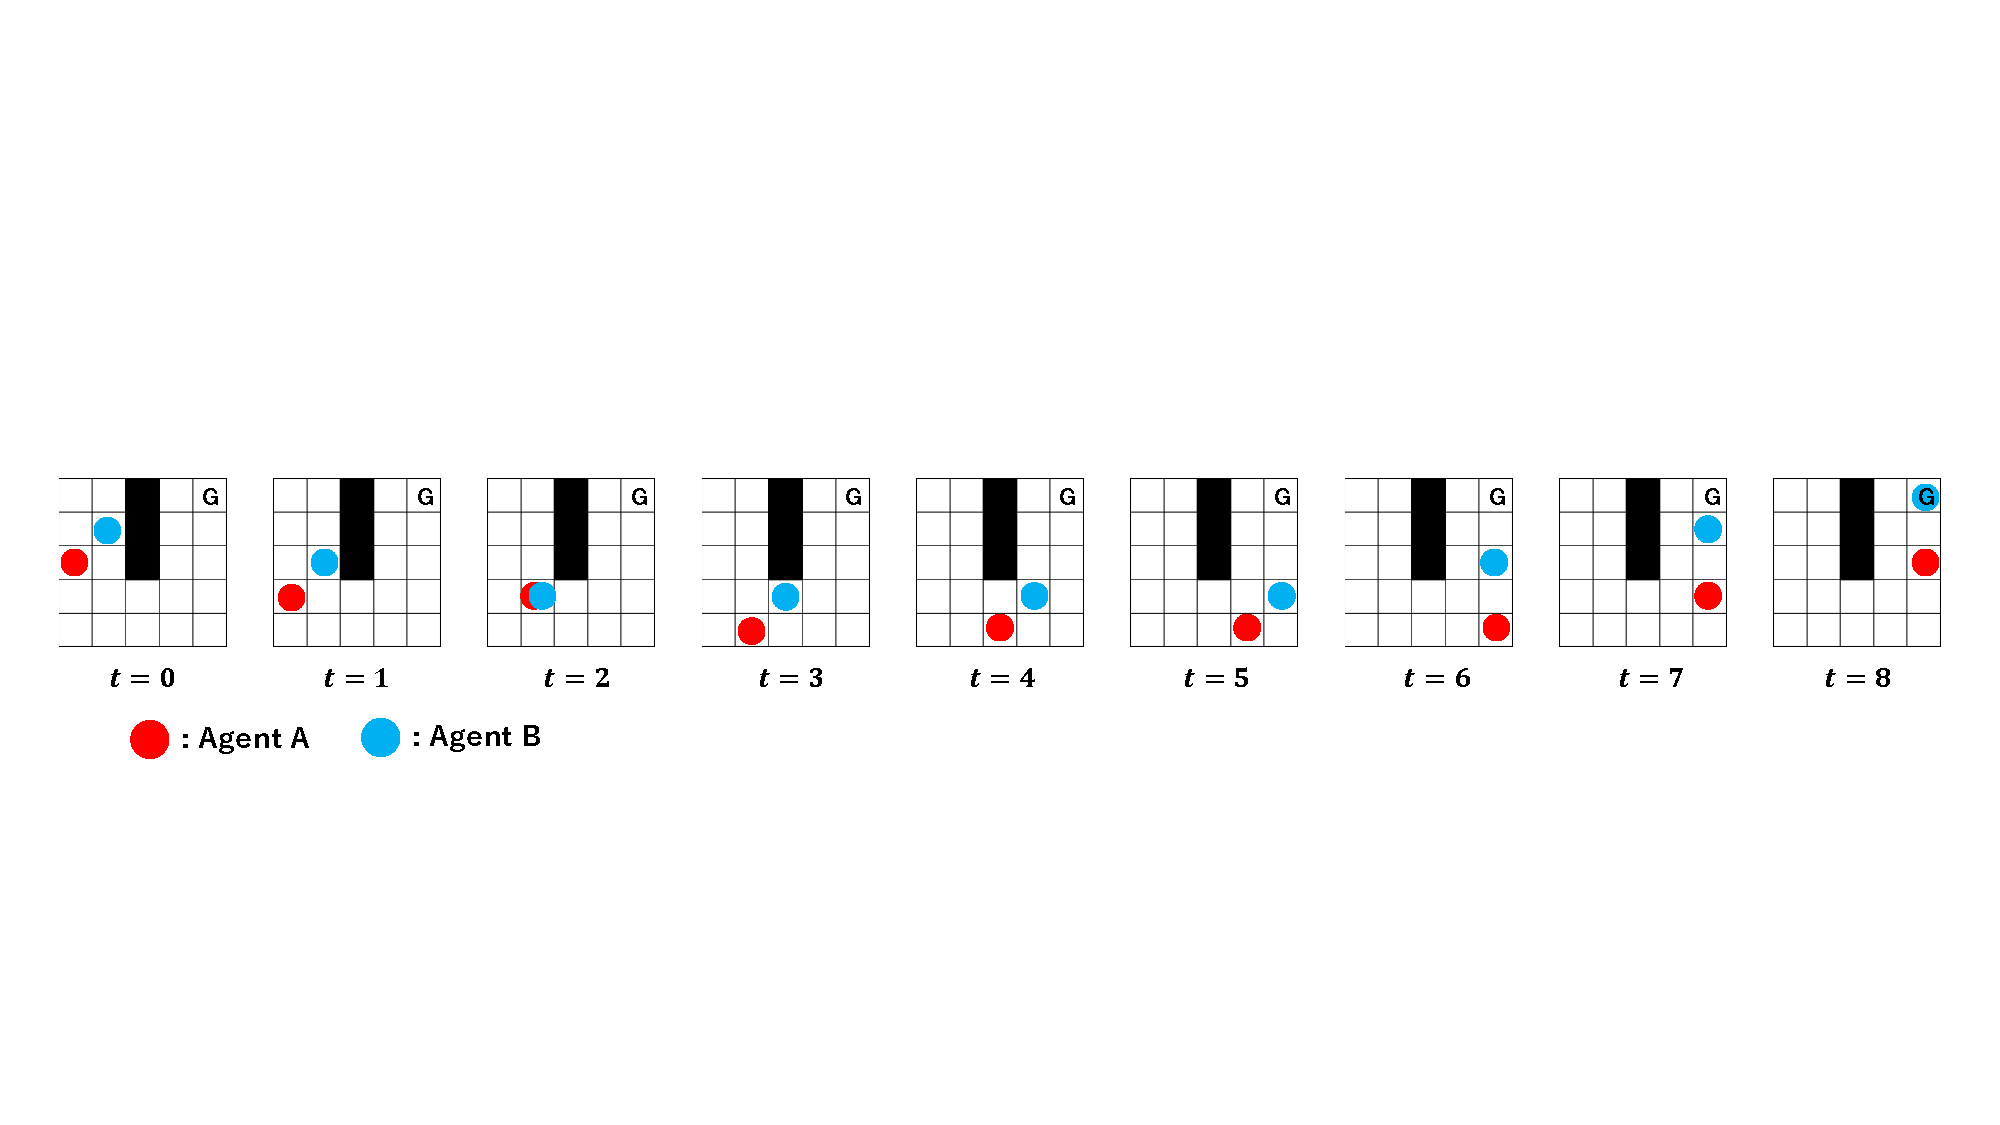
\includegraphics[scale=0.53]{fig/planning.pdf}
	\vspace{-10 mm}
	\caption{生成された行動の例}
	\label{fig:planning}
	\end{center}
\end{figure*}

\subsection{状態とメッセージに基づいた行動決定}
\label{2.2}
各エージェント$i \in \{A,B\}$は,自身の状態$s^t_{i}$と\ref{2.1}節で推論したメッセージ$m^t$に基づき,次式から行動$a^t_{i}$を選択する.
%
\begin{equation}
a^t_{i} \sim \pi_{i}(\cdot | s^t_{i}, m^t) \label{eq:action}
\end{equation}
%
$\pi_{i}$は各エージェントの方策を表す.
各エージェントはメッセージによって間接的に相手の状態を知ることができるため,自身と相手の状態に応じた行動を選択することができる.
%つまり,メッセージには両者の行動を変化させる役割があり,コミュニケーションによって協調を促すように両者の行動を調整できる.
また,選択した行動$a^t_{i}$に対する価値$v^t_{i}$は,次式の行動価値関数$Q_{i}$から算出される.
%
\begin{equation}
v^t_{i} = Q_{i}( s^t_{i}, a^t_{i}, m^t) \label{eq:value}
\end{equation}
%
$\pi_i$と$Q_i$をニューラルネットワークで近似したSoft Actor Criticを用いて,これらの関数を学習する.
ネットワークのパラメータ$\varphi_{i}$,$\theta_{i}$を用いて各エージェントの方策を$\pi_{\varphi_{i}}$,行動価値関数を$Q_{\theta_{i}}$と表すと,最小化する目的関数は次式となる.
%
\small
\begin{eqnarray}
J_{\pi}(\varphi_{i}) &=& E[ \alpha \log\pi_{\varphi_{i}}(a^t_{i} | s^t_{i}, m^t)-Q_{\theta_{i}}(s^t_{i},a^t_{i},m^t) ] \\ 
J_{Q}(\theta_{i}) &=& E[\frac{1}{2}(Q_{\theta_{i}}(s^{t}_{i},a^{t}_{i},m^{t}) - \hat{Q}(s^{t}_{i},a^{t}_{i},m^{t})^2]  
\end{eqnarray}
\normalsize
%
ただし
%
\small
\begin{equation}
\hat{Q}(s^{t}_{i},a^{t}_{i},m^{t}) = r^t_{i} + \beta r^t_{m} + \gamma E[V(s^{t+1}_{i}, m^{t+1})] \label{beta}
\end{equation}
%
\begin{equation}
V(s^t_{i}) = E [Q_{\theta_{i}}(s^{t}_{i},a^{t}_{i},m^{t}) - \alpha log \pi_{\varphi_{i}}(a^t_{i} | s^t_{i}, m^t) ]
\end{equation}
\normalsize
%
である.また,$\alpha$はエントロピー正則化への重み,$\beta$は協調行動の報酬の重み,$\gamma$は割引率である.
それぞれの目的関数が最小となるように,勾配降下法によって以下のようにパラメータを更新する.
%
\begin{equation}
\varphi_{i} 	\leftarrow \varphi_{i} - \lambda_{\varphi_{i}} \nabla_{\varphi_{i}} J_{\pi}(\varphi_{i})
\end{equation}
%
\begin{equation}
\theta_{i} 	\leftarrow \theta_{i} - \lambda_{\theta_{i}} \nabla_{\theta_{i}} J_{Q}(\theta_{i})
\end{equation}
%
ただし,$\lambda_{\varphi_{i}}, \lambda_{\theta_{i}}$は学習率である.





\section{現在の結果}
提案手法を用いて2体のエージェントが協調行動を学習できるかを検証した.
図\ref{fig:world}のグリッドワールド空間で,互いが衝突を回避しながらゴールへ到達することを目標とする移動タスクを行った.
%図\ref{fig:world}が実験に用いるグリッドワールドであり,番号が付いているグリッドが移動可能なグリッドである.
%両エージェントのゴールをどちらも3番のグリッドとし,互いが衝突を回避しながらゴールへ到達することを目標とする.
%状態$s$は,現在いるグリッドの番号の要素を$1$としたワンホットベクトルである.行動は$a \in \{0,1,2,3\}$で上下左右への移動を表している.報酬$r$は壁に衝突した場合は$-1$,
%移動可能グリッドにいる場合は$0$,ゴールへ到達した場合は$1$とした.協調行動の報酬$r_m$は,2体が同じグリッドにいる(衝突した)場合は$-1$,異なるグリッドにいる場合は$0$とした.
%メッセージ$m$は$64$次元のカテゴリカル変数であり,推論されたメッセージの要素を$1$としたワンホットベクトルである.

\subsection{モデルの学習}
\label{3.2}
本実験では,オフラインで事前に取得した学習データを用いてモデルを学習させた後に,協調行動が可能か検証した.
まず,各エージェントのスタート地点を数ヶ所設定してランダムに行動させ,一方がゴールに到達したらスタート地点に戻すことを繰り返し,
計9840個の学習データ$[s^t_{i},a^t_{i},s^{t+1}_{i},r^{t}_{i},r^{t}_{m}]$を取得した.
次に,取得したデータから,互いの状態と協調行動の関係を表現するメッセージ$m^t$をMHNGによって推論した.
推論されたメッセージも加えたデータ$[s^t_{i},a^t_{i},s^{t+1}_{i},r^{t}_{i},r^{t}_{m},m^t]$を用いたミニバッチ学習により,方策$\pi_{i}$と行動価値関数$Q_{i}$を学習した.
%学習時の各パラメータを表\ref{tbl:train_params}に示す.
%また,MH名付けゲームによって生成されたメッセージの一部を図\ref{fig:msg}に示す.
%図\ref{fig:msg}中の$p(s_{A}|m),p(s_{B}|m),p(r_{m}|m)$は,各メッセージが表現する確率分布である.
%$m=0$のメッセージは,互いが異なる位置にいて協調できていることを表現している.
%対して$m=1$のメッセージは,互いが同じ位置にいて衝突していることを表現している.
%このことから,コミュニケーションによって互いの状態を適切に表現するメッセージを学習できたといえる.

%実験環境
\begin{figure}[t]
\centering
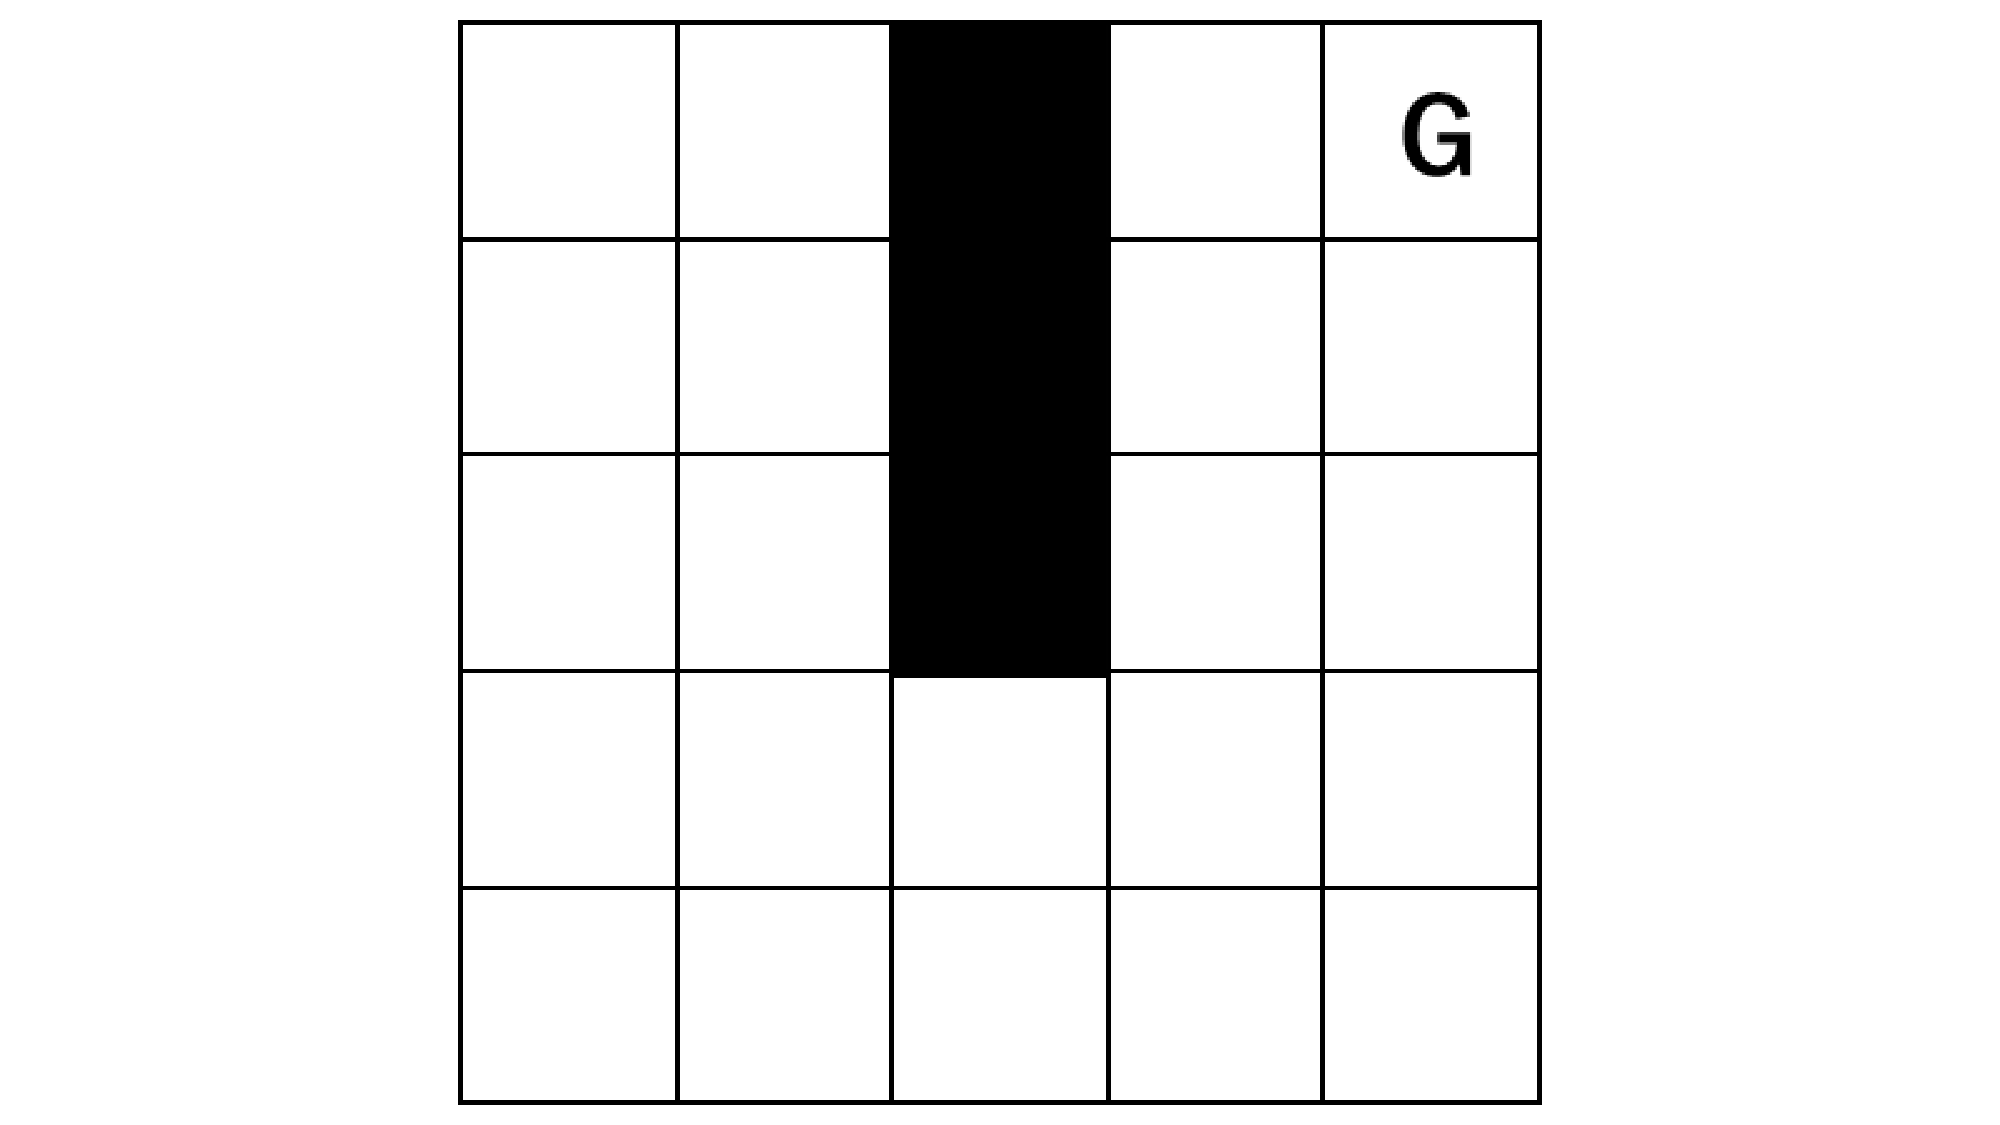
\includegraphics[scale=0.2]{fig/world.pdf}
\caption{実験環境}
\label{fig:world}
\end{figure}


\subsection{協調行動の生成}
\label{3.3}
学習されたパラメータを用いて,両エージェントが協調してゴールに到達できるかを検証した.
まず各エージェントを移動可能グリッドにランダムに配置し,各状態に対するメッセージをMHNGによって推論した.
次に,状態と推論したメッセージを各Actorに入力し,出力された行動を実行して次の状態を決定した.
以降は同様に,各状態に対するメッセージの推論と行動生成をゴールに到達するまで繰り返した.
この手順を1000回繰り返し,スタートからゴールするまでの衝突回数の合計を算出した.
%また,比較として,メッセージなしの場合で\ref{3.2}節と同様の条件で学習したモデルを利用し,行動生成を行った.
実験結果を表\ref{res}に示す.
表\ref{res}より,メッセージなしの場合と比較して,衝突回数が約75\%減少していることが分かる.
%これは,コミュニケーションによって互いの状態を伝達したことで,互いが衝突しない行動を学習できたためだと考えられる.
また,スタートからゴールまでの生成された行動の例を図\ref{fig:planning}に示す.
%図\ref{fig:planning}より,$t=2$では互いが衝突してしまっているものの,$t=3$でエージェントAが衝突を避ける方向へ移動し,その後再びゴールに向かっていることが分かる.
図\ref{fig:planning}より,途中で一度衝突したものの,そこからエージェントAが衝突を避ける方向へ移動し,その後再びゴールに向かっていることが分かる.
%これは,メッセージによってエージェントAの行動が変化したためだと考えられる.
このことから,両エージェントが状況に応じて協調行動しつつ,ゴールに向かう方策を学習できていることが確認できる.

\begin{table}[t]
\caption{実験結果}
\label{res}
\centering
\scalebox{0.92}{
\begin{tabular}{c c c} \hline
\rule[-1pt]{0pt}{10pt} & メッセージ$m$あり &  メッセージ$m$なし \\ \hline
\rule[-1pt]{0pt}{10pt} 衝突回数(回) \rule[-1pt]{0pt}{10pt} & 66 & 252 \\ \hline
\end{tabular}
}
\end{table} 

%%%%%%%%%%%%%%%%%%%%%%%%%%%%%%%%%%%%%%%%%%%%%%%%%%%%%%%%%%%%%%%%%%%%%%%%%%%%%%%%%%%%%%%%%
\section{まとめ及び今後の取り組み}
本稿では,MHNGと深層強化学習を組み合わせることで,協調行動の学習が可能なモデルを提案した.
実験では,エージェント同士がメッセージを介したコミュニケーションにより,互いの状態に応じて衝突を回避した行動を学習できることを確認した.
今回は状態・行動が離散なタスクで評価したが,今後は状態・行動が連続なタスクへ適用することを考えている.
また,潜在状態空間モデルへ拡張し,実世界のロボットタスクに適応することを目標としている.
%
%%%%%%%%%%%%%%%%%%%%%%%%%%%%%%%%%%%%%%%%%%%%%%%%%%%%%%%%%%%%%%%%%%%%%%%%%%%%%%%%%%%%%%%%%
\vspace*{-0.55cm}
\small
\begin{thebibliography}{99}
%MH naming game
\bibitem{mh1}
Tadahiro Taniguch et al., ``Emergent Communication through Metropolis-Hastings Naming Game with Deep Generative Models'', arXiv: 2205.12392, 2022.

%NakamuraLab
\bibitem{ebara}
江原広人, 中村友昭, 谷口彰, 谷口忠大, ``分散的ベイズ推論としてのマルチエージェント強化学習と記号創発'', 言語処理学会第29回年次大会, 2023

\bibitem{nakamura}
Tomoaki Nakamura, Akira Taniguchi, Tadahiro Taniguchi, ``Control as Probabilistic Inference as an Emergent Communication Mechanism in Multi-Agent Reinforcement Learning'',arXiv:2307.05004, 2023


\end{thebibliography}
%
\thispagestyle{fancy}
\renewcommand{\headrulewidth}{0.0pt}

\end{document} 